\section{Ejercicio 8}

Presentamos el siguiente lote corrido con distintos semillas de aleatoridad y tamaño de quantum.

TaskBatch 10 1 \\
TaskBatch 20 1 \\
TaskBatch 13 3 \\
TaskBatch 17 1 \\
TaskBatch 27 1 \\
TaskBatch 11 2 \\

\begin {center}
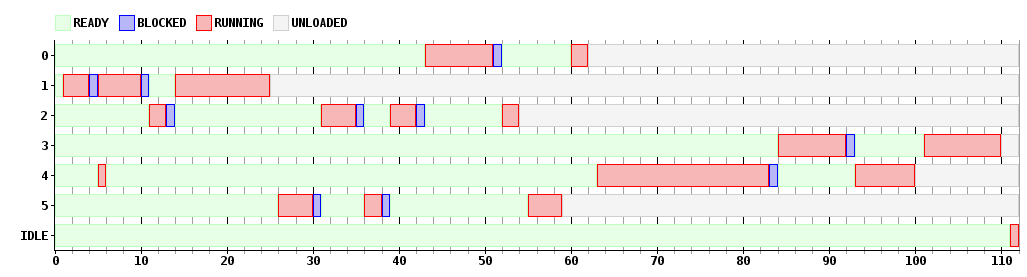
\includegraphics[width=16cm]{../simusched/outputs/loterya.png}
\end {center}
\begin {center}
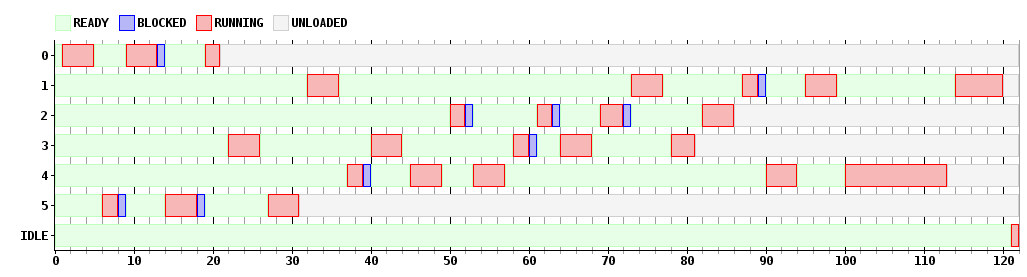
\includegraphics[width=16cm]{../simusched/outputs/loteryc.png}
\end {center}
\begin {center}
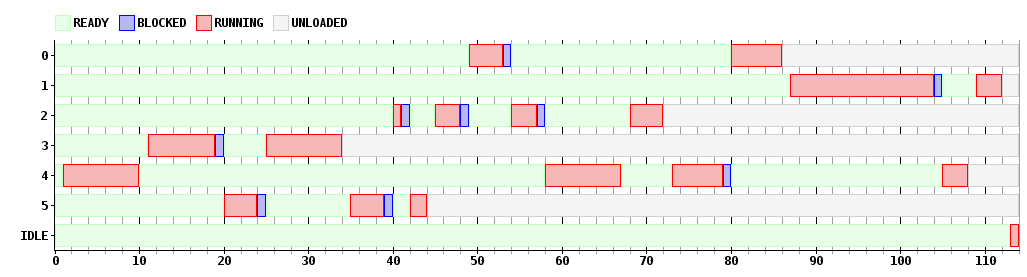
\includegraphics[width=16cm]{../simusched/outputs/loteryd.png}
\end {center}
\begin {center}
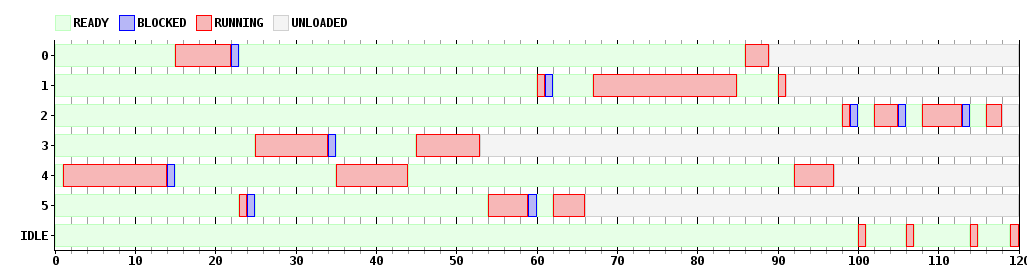
\includegraphics[width=16cm]{../simusched/outputs/loterye.png}
\end {center}
\begin {center}
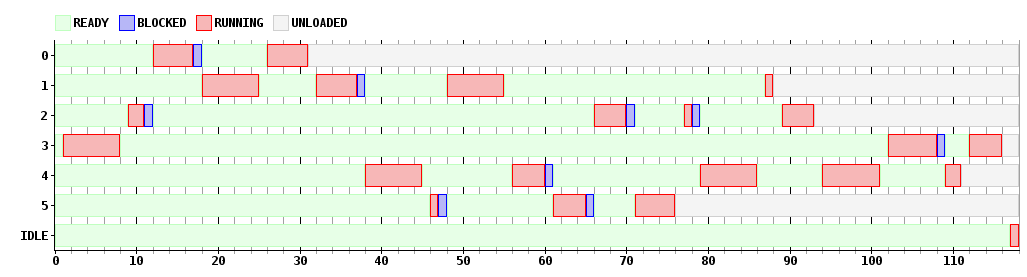
\includegraphics[width=16cm]{../simusched/outputs/loteryf.png}
\end {center}



Se puede notar que aunque se elija el mismo lote, la aleatoridad del algoritmo muestra como aunque se asignen de distinta forma los recursos, todos los procesos
tienden a obtenerlos uniformemente.\\
Utilizamos el mismo ejemplo para notar la $"$compensación$"$. Notese como en el A el proceso 1 después de haber bloqueado 2 veces obtuvo tantos tickets que casi tuvo
exclusividad del procesador. Por el contrario el proceso 4 tuvo que esperar varios sorteos hasta salir ganador.
